\IEEEraisesectionheading{\section{Introduction}\label{sec:introduction}}


Remarkably,
%%SL.09.03: I think starting with a superlative doesn't quite set the right tone.
humans are able to learn a range of complex yet generalizable behaviors when faced with a stream of high-dimensional sensory inputs and minimal external supervision. The reinforcement learning (RL) problem statement covers such a real-world setting. Yet, the general setting of learning from raw sensory inputs from sparse rewards in the real world is incredibly challenging. To make progress, many prior works have chosen various assumptions to make the problem more tractable. For instance, some works have been demonstrated only in settings where shaped rewards are available~\cite{todo}.
%%SL.09.03: I don't think it's a good idea to start the very first paragraph with something so negative. We can discuss previous work later, the first paragraph should start on a positive note about how prediction is often considered a fundamental component of intelligence.
Others have assumed access to a perfect or hand-engineered simulator, from which millions of roll-outs can be taken~\cite{atari,openai_hand}.
A few works have assumed that a low-dimensional, compact state representation is accessible during training~\cite{e2e,asymmetric_ac}. Finally, many works reset the state between roll-outs to a relatively narrow distribution of initial states, leading to a task is more repeatable~\cite{atari,dsae,gps,etc}.
%%SL.09.03: seems way too low-level for the first paragraph. We should also leave all the buzzwordy stuff (alphago, atari, etc) for later, it really has little to do with the main topic of the paper.
By making such assumptions, these prior methods have demonstrated the ability to learn complex visuomotor skills~\cite{e2e}, learn Atari games from pixels~\cite{atari}, and master the game of Go~\cite{alphago}.
%% CF: I don't like using "real-world" so much below, because we are still in a lab environment... thoughts?
However, to move these algorithms towards achieving general behaviors in the real world, it is arguably necessary to deploy them in diverse, real-world environments.
Unfortunately, it is challenging to deploy such methods for learning in diverse, real-world environments, where shaped rewards, resets, compact state representations, and simulations are largely unavailable without extensive human involvement.

Unlike many prior works that focus on RL for mastery of highly-specialized skills in closed-world environments, here we instead focus on \emph{generalization} in diverse environments.
%%SL.09.03: this is an important and critical sentence, but I don't like that we from the outset present it in contrast to something so negative (those other guys fail at this, but we don't) -- just say what we do well, and then talk about alternatives. I think we can motivate the work and explain the challenge without necessarily getting so bogged down in the failure of prior work.
We consider a robotic control domain with a wide range of objects, where the algorithm has access to only raw sensor observations (i.e. pixels) and sparse rewards and has minimal control over the environment and how it can be reset. In such a setting with minimal assumptions, rewards are simply not enough supervision
%%SL.09.03: I think this is not quite capturing the point. I think it will be easier to motivate learning w/o rewards from an analogy to how humans learn, instead of by saying that assumptions of prior work are bad. Then we can talk about assumptions of prior work afterwards.
to be learned from alone. Instead, the supervision needs to come from the observations themselves. As such, we propose to learn action-conditioned predictive models directly on raw pixel observations.
%%SL.09.03: well, we do more than learn such models, we show that they can accomplish complex manipulation tasks on real-world robots
Beyond the necessity of dense supervision, observation models have two additional benefits. They are goal-agnostic, which enables learning for a variety of different goals; and, by learning on top of raw observations, they are fully general in that they do not require a hand-engineered representation of the environment.
%%SL.09.03: again, let's leave the negativity for later

%In addition the practicality of leveraging the only available supervision in such sparse reward environments, observation models are also goal-agnostic, which enables learning for a variety of different goals.
%% TODO - motivate why not to learn a model on top of a more abstract representation of the observations? [The supervision, inherently, comes from the same place.]
%TODO - motivate why raw pixels rather than more compact representation (because pixels contain complete information -- can give Sergey's crossing-the-street example -- and pixels are the only thing that is readily available; also pixels contain more supervision)

\begin{figure}[t]
\centering
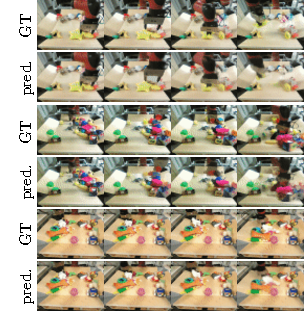
\includegraphics[width=.8\columnwidth,trim={3.2mm 0 0 0},clip]{images_rfr/video_prediction.pdf}
\caption{\small{\todo{Overview of visual MPC concept}}}
\label{fig:video_prediction}
\end{figure}
%%SL.09.03: the figure looks awkwardly stretched, and it's not clear what the robot is actually doing

Despite the benefits, a number of challenges arise when aiming to use observation models: how can we learn a model of high-dimensional observations? how should an objective or reward be determined with respect to the predicted observations? how should experience be collected? how should actions be chosen with respect to the model? We discuss each of these design decisions and propose several options, weighting the benefits and trade-offs of each.
%%SL.09.03: sounds a bit too much like a laundry list, can we pull some broader themes and dive into details later?
Our overall approach amounts to a deep model-based reinforcement learning algorithm that leverages video prediction models to achieve a variety of pixel-based control tasks without shaped reward information.

The main contributions of this work are as follows. First, we propose a general framework for deep reinforcement learning with observation models, abstracting away design decisions such as the model, the policy optimization, and the reward function.
%%SL.09.03: seems reasonable, but when we abstract away so much, we just get the classic model-based RL problem setting. Maybe this is a little bit too much abstraction.
Second, we propose a model that can better maintain object permanence through occlusions via temporal skip connections.
%%SL.09.03: I wouldn't put this "Second" -- maybe something more general like architectures for prediction?
Third, we discuss several forms of planning objectives, including goal pixel positions, goal image registration, and image classifiers.
%%SL.09.03: without motivation, this seems a bit arbitrary. I think this is a good contribution, but the phrasing makes it seem like a less significant detail somehow.
Finally, our evaluation demonstrates that these components can be combined to enable a real robot to perform a range of real-world object manipulation tasks from raw pixel observations. Our experiments include manipulation of previously unseen objects, handling multiple objects, pushing objects around obstructions, handling clutter, recovering from large perturbations, and grasping and maneuvering objects to user-specified locations in 3D-space. These results represent a significant advance in the \emph{generality} of skills that can be acquired by a real robot operating on raw pixel values.

This paper builds upon prior conference papers~\cite{todo}; our new contributions include an empirical evaluation of cloth manipulation and/or stochastic models, analysis of each method involving XX, as well as a comprehensive, open-sourced simulation environment to facilitate future research and better reproducibility.




\todo{make big VMPC diagramm!!}


\iffalse

current approaches for general-purpose robotic manipulation can be loosely categorized into two schools: The first where algorithms are designed, trained or tuned in simulation and then deployed in the real world. While simulation has the advantage of being cheaper and running orders of magnitudes faster it also often comes at a price: Many real-world phenomena such as complex friction, soft-objects, liquids or even other agents such as humans often cannot be modeled with sufficient fidelity. Therefore the resulting policies often do not transfer very well from simulation the real world.

A completely different approach is to avoid simulation and manual feature engineering and instead learn models and policies through interacting with the real world. This typically requires human resets and complex hand-engineered reward functions. For example \cite{DBLP:journals/corr/GuHLL16} presents a method for learning door opening using robot manipulators in the real world while humans are required to perform hundreds of resets in addition to sensors measuring the success of the door opening task.

Here we present a family of methods (extending our work in \cite{foresight}, \cite{sna}, \todo{cite robustness from retry, SAVP, classifier VMPC}) that enable robots to learn complex manipulation skills from interacting with their environment requiring \emph{very little or no human supervision at all}. We show that the need for human supervision can be removed by training an action-conditioned video-prediction model from data that is collected completely autonomously by the robot interacting with its environment. This work demonstrates that by training the model on the task of predicting what it will see next (for a given sequence of motor commands) it learns models of environment dynamics that can be used effectively for robotic control.

In the proposed approach neither models of the robot nor the environment dynamics need to be provided ahead of time, since the action-conditioned prediction model is learned purely on autonomously collected data.

For video-prediction-based control a specific type of model -- transformation-based video-prediction -- has proven to be particularly effective. One of the reasons is that the transformations can be used to obtain predictions of \emph{where} certain pixels in the image are moving. However due to occlusion (of objects by the arm) severe limitations for planning performance can arise when planning costs are computed from transformation-based predictions. We propose type of video-prediction model that uses temporal skip connections to recover parts of the images that are occluded during the predictions and demonstrates that this yields significant improvements for manipulation planning.
\fi


\iffalse

\todo{mention stochastic video prediction in case improvements are observed}

To achieve complex long-term behaviour the ability to correct for mistakes due to uncertainty and accumulating erros in the models predictions is a key requirement. If the agent can always evaluate the goal (along its predictions), it can continuously retry, so that even flawed predictions allow for an eventual successful execution. To this end we propose a cost function for video-prediction based planning based on image registration, which we demonstrate can itself be learned on the same dataset as the one used to train the predictive model. This closed-loop visual control allows the robot to be persistent, correcting for mistakes caused by inevitable model inaccuracies allowing it to retry indefinitely until it succeeds.

\todo{motivate one-shot classifier based control}

The technical contribution of this work is four-fold. First, we present a video-prediction-based method for robotic control that enables learning complex manipulation skills \emph{purely from autonomously collected data}. Second we show that the video-prediction model's capability to \emph{accurately maintain object permanence through occlusions} can be enhanced by incorporating temporal skip connections. Third we propose a method for allowing \emph{closed loop control} equipping the agent with the ability to retry the task indefinitely until it succeeds which contributes significantly to the method's robustness. Fourth a cost function based on a few-shot classifier-based is presented which allows the agent to successfully \emph{execute tasks defined by a single demonstration}.

Our evaluation demonstrates that these components can be combined to enable a learned video prediction model to perform a range of real-world pushing tasks. Our experiments include manipulation of previously unseen objects, handling multiple objects, pushing objects around obstructions, and moving the arm around and over other obstacle-objects, recovering from large perturbations, grasping objects and maneuvering them to a user-specified point in 3D-space representing a significant advance in the range and complexity of skills that can be acquired through entirely self-supervised learning.

\fi

 





